\documentclass[tikz,border=8pt]{standalone}
\usepackage{ctex}
\usepackage{amsmath}
\usetikzlibrary{calc, arrows.meta}

\begin{document}
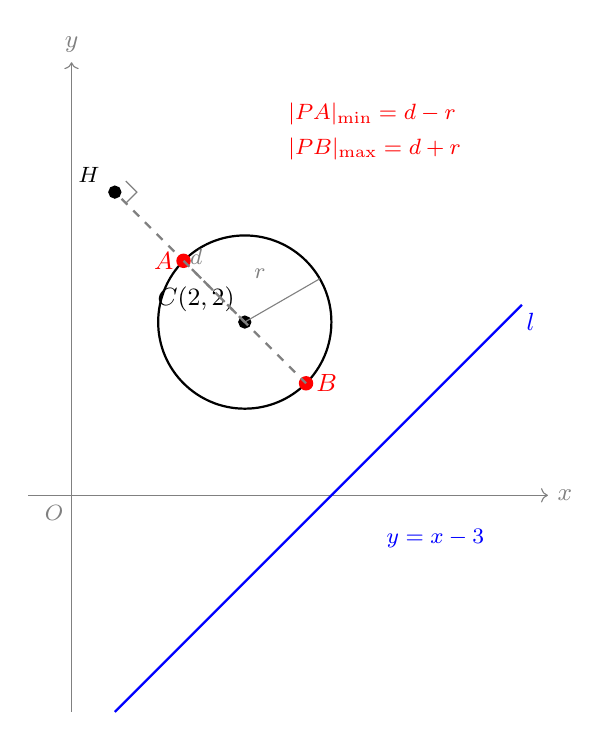
\begin{tikzpicture}[scale=1.1, thick]

% 坐标轴
\draw[->, thin, gray] (-0.5,0) -- (5.5,0) node[right, font=\small, gray] {$x$};
\draw[->, thin, gray] (0,-2.5) -- (0,5.0) node[above, font=\small, gray] {$y$};
\node[font=\footnotesize, gray] at (-0.2,-0.2) {$O$};

% 圆心 C(2,2)，半径 r=1
\coordinate (C) at (2,2);
\draw[black, thick] (C) circle [radius=1];
\filldraw[black] (C) circle (1.8pt);
\node[font=\small, above left] at (C) {$C(2,2)$};

% 直线 y = x - 3，即 x - y - 3 = 0
% 两点：x=1→y=-2；x=5→y=2
\draw[blue, thick] (0.5,-2.5) -- (5.2,2.2);
\node[blue, font=\small] at (5.3, 2.0) {$l$};
\node[blue, font=\footnotesize] at (4.2, -0.5) {$y=x-3$};

% 圆心到直线距离
% d = |2 - 2 - 3|/sqrt(2) = 3/sqrt(2) = 3√2/2 ≈ 2.121
% 法向量方向（直线 x-y-3=0，法向量 (1,-1)/√2）
% 垂足 H = C - d*(1,-1)/√2  （朝直线方向）
% H = (2,2) - (3/2)*(1,-1) = (2-1.5, 2+1.5) = (0.5, 3.5)
\coordinate (H) at (0.5, 3.5);

% 画垂线 CH（灰色虚线，标 d）
\draw[gray, dashed, thick] (C) -- (H);

% 垂足在直线上的标记
\filldraw[black] (H) circle (1.8pt);
\node[font=\footnotesize] at (0.2, 3.7) {$H$};

% 直角标记
% CH 方向：(0.5-2, 3.5-2)=(-1.5,1.5)，单位化 (-1/√2, 1/√2)
% l 方向：(1,1)/√2
\draw[gray, thin]
  ($(H) + 0.18*({1/sqrt(2)},{1/sqrt(2)})$) --
  ($(H) + 0.18*({1/sqrt(2)},{1/sqrt(2)}) + 0.18*({1/sqrt(2)},{-1/sqrt(2)})$) --
  ($(H) + 0.18*({1/sqrt(2)},{-1/sqrt(2)})$);

% 圆上最近点 A（C 沿 CH 方向移动 r）
% CH 方向单位向量：(-1/√2, 1/√2)
% A = C + 1*(-1/√2, 1/√2) = (2-0.707, 2+0.707) = (1.293, 2.707)
\coordinate (A) at ({2-1/sqrt(2)}, {2+1/sqrt(2)});
\filldraw[red, thick] (A) circle (2pt);
\node[red, font=\small, left] at (A) {$A$};

% 圆上最远点 B（C 沿 HC 方向移动 r）
% B = C + 1*(1/√2, -1/√2) = (2+0.707, 2-0.707) = (2.707, 1.293)
\coordinate (B) at ({2+1/sqrt(2)}, {2-1/sqrt(2)});
\filldraw[red, thick] (B) circle (2pt);
\node[red, font=\small, right] at (B) {$B$};

% 延长线（从 A 到 B 穿过圆心）
\draw[gray, dashed] (A) -- (B);

% 标 d（圆心到直线距离）
\node[font=\footnotesize, gray, right] at ($(C)!0.5!(H)$) {$d$};

% 标注最小最大值
\node[font=\footnotesize, align=left, red] at (3.5, 4.2) {
  $|PA|_{\min}=d-r$\\[3pt]
  $|PB|_{\max}=d+r$
};

% r 标注
\draw[gray, thin] (C) -- ({2+cos(30)},{2+sin(30)});
\node[font=\footnotesize, gray] at ({2+0.35*cos(60)},{2+0.35*sin(60)+0.25}) {$r$};

\end{tikzpicture}
\end{document}
